\documentclass[10pt, compress]{beamer}

% Tema de la presentación
\usetheme[usetitleprogressbar, usetotalslideindicator]{m}

% Tabla de contenidos precedida de ∙
\setbeamertemplate{section in toc}{%
    ∙  \inserttocsection \par}

% Mejora de las tablas
\usepackage{booktabs}

% Inclusión de gráficos
\graphicspath{{./graphics/}{./graphics/screenshots/}}

% Extensiones de gráficos
\DeclareGraphicsExtensions{.pdf,.jpeg,.jpg,.png}

% Renderizado de la fecha
\usepgfplotslibrary{dateplot}

% Título
\title{Interfaz web para la gestión de sondas de red de altas prestaciones}
% Subtítulo
% \subtitle{Trabajo de Fin de Grado}
% Fecha
\date{Junio 2015}
% Autor
\author{Juan Sidrach de Cardona Mora}
% Grupo de investigación
\institute{High-Performance Computing and Networking}

% Contenido
\begin{document}

% Portada
\maketitle

% Tabla de Contenidos
\begin{frame}{Tabla de Contenidos}
 \tableofcontents
\end{frame}

% Introducción
\section{Introducción}

% Sondas de red
\begin{frame}{Sondas de red}
  \begin{itemize}
    \item\alert<+>{Dispositivos capaces de capturar y/o inyectar tráfico de red}
    \item\alert<+>{Principales usos}
    \begin{itemize}
      \item Análisis de las trazas capturadas por la sonda
      \item Realización de pruebas sobre redes, plataformas y aplicaciones
    \end{itemize}
    \item\alert<+>{Diferentes tipos sobre ordenadores convencionales}
    \begin{itemize}
      \item Tarjetas Ethernet estándar
      \item Tarjetas a medida basadas en FPGAs
    \end{itemize}
  \end{itemize}
\end{frame}

% Sonda utilizada
\begin{frame}{Sonda utilizada}
  \begin{itemize}
    \item\alert<+>{Sonda a medida basada en FPGA}
    \item\alert<+>{Permite capturar y reproducir tráfico de red}
    \item\alert<+>{Rendimiento máximo de 10 Gbps}
    \begin{itemize}
      \item Puede verse limitado por la velocidad del disco
    \end{itemize}
    \item\alert<+>{Gestionada por línea de comandos}
  \end{itemize}
\end{frame}


% Estado del arte
\section{Estado del arte}

% OSNT
\begin{frame}{The Open Source Network Tester}
  \begin{itemize}
    \item\alert<+>{Sistema de captura y reproducción de código abierto}
    \item\alert<+>{Utiliza cuatro FPGAs}
    \begin{itemize}
      \item Mismo modelo que la empleada en este TFG
    \end{itemize}
    \item\alert<+>{Gestionadas desde una interfaz sobre el propio servidor}
    \item\alert<+>{Se han identificado algunos aspectos mejorables}
    \begin{itemize}
      \item Provee información exclusivamente de la FPGA
      \item Interfaz poco intuitiva
      \item Se maneja desde el propio servidor
    \end{itemize}
    \item\alert<+>{Otras aplicaciones consideradas}
    \begin{itemize}
      \item tcpdump/libpcap
      \item Wireshark
      \item Detect-Pro
    \end{itemize}
  \end{itemize}
\end{frame}

% OSNT - Interfaz
\begin{frame}{The Open Source Network Tester - Interfaz}
  \begin{figure}
    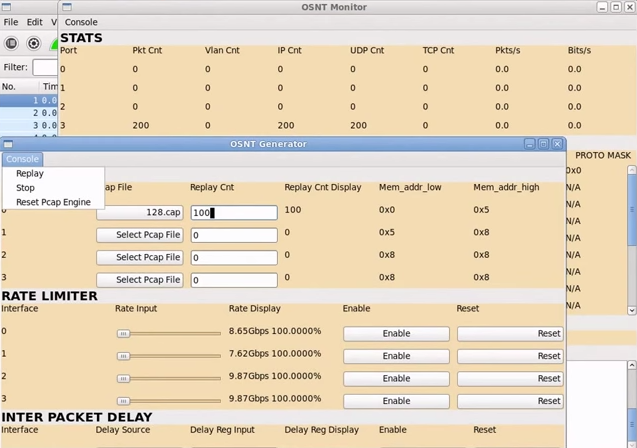
\includegraphics[width=0.9\linewidth]{osnt}
  \end{figure}
\end{frame}


% Definición del proyecto
\chapter{Definición del proyecto\label{cap:defProyecto}}

En este capítulo se definirán y explicarán el alcance del proyecto, la metodología de desarrollo escogida y las herramientas utilizadas.

\section{Alcance\label{sec:dp:alcance}}

Esta aplicación tiene como objetivo permitir, mediante una interfaz web, gestionar una sonda de red y conocer su estado actual.
Asimismo, posibilitará manejar otros aspectos relacionados con la sonda, como el almacenamiento y gestión de las \glspl{traza} capturadas.
Estos aspectos son comunes a cualquier sistema de captura y reproducción de tráfico de red, por lo que se estructurará la aplicación de forma que generalice el problema dado, sirviendo como trabajo base para la creación de interfaces gráficas sobre sondas similares.

No se pretende sin embargo, dentro del contexto de este proyecto, que la interfaz web sea capaz de interactuar con cualquier tipo de sonda de captura y reproducción de tráfico de red, sino solo con la sonda seleccionada.
Tampoco entra dentro del alcance de este proyecto modificar el funcionamiento interno de la sonda, ni siquiera para mejorar su rendimiento, ya que el objetivo principal es facilitar la gestión de una sonda de red de altas prestaciones y de otros componentes que intervienen en el sistema.

\section{Metodología\label{sec:dp:metodologia}}

Para el desarrollo de la aplicación se ha optado por seguir un ciclo de vida en cascada con retroalimentación.
Este modelo ordena las etapas del proceso de desarrollo software, de forma que solo se pueda iniciar una fase cuando se ha finalizado la anterior.
Dada la naturaleza de este proyecto, era necesario un periodo amplio de estudio del problema a resolver antes de poder codificar nada, siendo por ello este modelo más recomendable que adoptar alguna metodología ágil.
Por otra parte, se ha descartado utilizar un modelo iterativo o en espiral dado que conllevaría un mayor tiempo de desarrollo al tener que realizarse por módulos y de forma separada cada una de las fases definidas, en vez de simultáneamente y de forma global.
Además, el hecho de tener retroalimentación permite volver a etapas anteriores en caso de que sea necesario corregir algún aspecto del sistema.

La distribución temporal de las tareas y sus dependencias se resumen en el diagrama de Gantt de la Figura~\ref{fig:gantt}.
A continuación se detallan la entradas, tareas y salidas de cada una de las fases del desarrollo del proyecto.

\begin{figure}[!htp]
  \centering
  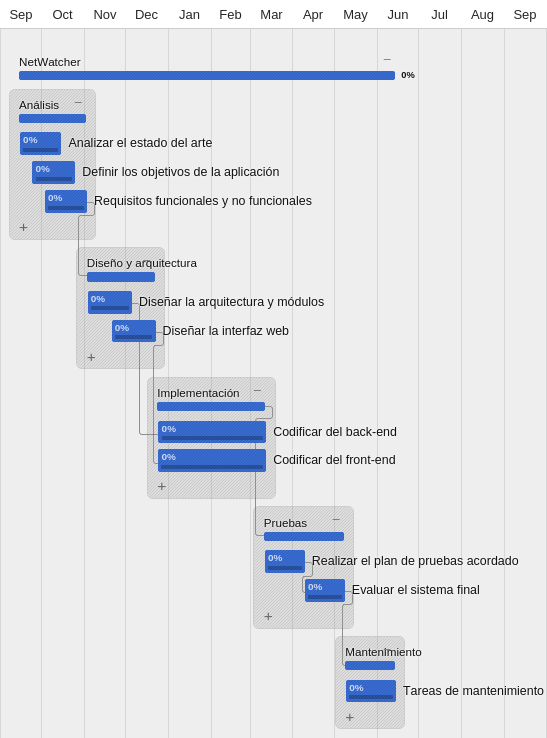
\includegraphics[width=0.7\textwidth,clip=true]{graphics/gantt_white}
  \caption{Diagrama de Gantt de la planificación temporal del proyecto}
  \label{fig:gantt}
\end{figure}

\subsection*{Análisis\label{ssec:dp:analisis}}

Tareas
\begin{itemize}[leftmargin=3.5em]
  \item Analizar el estado del arte.
  \item Definir los objetivos de la aplicación.
  \item Especificar los requisitos funcionales y no funcionales.
\end{itemize}

Salida
\begin{itemize}[leftmargin=3.5em]
  \item Definición, objetivos y alcance del proyecto.
  \item Relación de requisitos.
\end{itemize}

\subsection*{Diseño y arquitectura\label{ssec:dp:disenho}}

Entrada
\begin{itemize}[leftmargin=3.5em]
  \item Relación de requisitos.
\end{itemize}

Tareas
\begin{itemize}[leftmargin=3.5em]
  \item Diseñar la arquitectura y módulos a implementar.
  \item Diseñar la interfaz web.
\end{itemize}

Salida
\begin{itemize}[leftmargin=3.5em]
  \item Arquitectura de la aplicación.
  \item Diagramas de diseño.
  \item Maquetas de la interfaz web.
\end{itemize}

\subsection*{Implementación\label{ssec:dp:implementacion}}

Entrada
\begin{itemize}[leftmargin=3.5em]
  \item Información sobre la arquitectura y el diseño de la aplicación.
  \item Maquetas de la interfaz web.
\end{itemize}

Tareas
\begin{itemize}[leftmargin=3.5em]
  \item Codificar del \gls{back-end}.
  \item Codificar del \gls{front-end}.
\end{itemize}

Salida
\begin{itemize}[leftmargin=3.5em]
  \item Código de la aplicación.
  \item Documentación del código de la aplicación.
\end{itemize}

\subsection*{Pruebas\label{ssec:dp:pruebas}}

Entrada
\begin{itemize}[leftmargin=3.5em]
  \item Código de la aplicación.
\end{itemize}

Tareas
\begin{itemize}[leftmargin=3.5em]
  \item Realizar el plan de pruebas acordado.
  \item Evaluar el sistema final.
\end{itemize}

Salida
\begin{itemize}[leftmargin=3.5em]
  \item Código de la aplicación validado y verificado.
\end{itemize}

\subsection*{Mantenimiento\label{ssec:dp:mantenimiento}}

Entrada
\begin{itemize}[leftmargin=3.5em]
  \item Código de la aplicación validado y verificado.
\end{itemize}

Tareas
\begin{itemize}[leftmargin=3.5em]
  \item Analizar, implementar y probar las solicitudes de mejoras propuestas por usuarios.
\end{itemize}

Salida
\begin{itemize}[leftmargin=3.5em]
  \item Código de la aplicación validado y verificado, con cambios menores propuestos por usuarios.
\end{itemize}


\section{Herramientas\label{sec:dp:herramientas}}

Para el desarrollo de este proyecto han sido necesarias herramientas que cubran las siguientes necesidades:

\begin{itemize}
  \item Control de versiones.
  \item Creación de diagramas y maquetas.
  \item Documentación de la aplicación.
  \item Plataforma base para el \gls{back-end}.
  \item Plataforma base para el \gls{front-end}.
\end{itemize}

A continuación se especifican las herramientas elegidas, exponiendo su utilidad.
Se detallan también otras librerías externas de las que hace uso la aplicación.

\subsection*{Control de versiones: GitHub\label{ssec:dp:github}}

En todo proyecto software es fundamental, especialmente si se alarga en el tiempo, hacer uso de una herramienta de control de versiones para el código y la documentación.
Se ha elegido con este propósito utilizar la plataforma \textit{GitHub}~\cite{github}, basada en \textit{git}~\cite{git}, un sistema distribuido de control de versiones.
Esta plataforma es la más popular dentro de las herramientas de control de versiones, y tiene algunas ventajas importantes respecto a otros sistemas similares.

En primer lugar, ofrece alojamiento gratuito para proyectos de \gls{codigoabierto}, y también para proyectos privados si se es estudiante.
Gracias a esto se ha podido desarrollar todo el código de la aplicación en un proyecto privado, liberándolo al público al finalizar el desarrollo principal, de forma que cualquiera pueda utilizar y mejorar el código existente.
Por otra parte, \textit{GitHub} añade a la funcionalidad de \textit{git} la posibilidad de crear una \textit{wiki} del proyecto de forma sencilla, característica que ha sido utilizada en el proyecto.
Finalmente, facilita la colaboración entre desarrolladores con una interfaz intuitiva y cuya curva de aprendizaje no tiene una una pendiente demasiado elevada.

\subsection*{Creación de diagramas y maquetas: Cacoo\label{ssec:dp:cacoo}}

Para el diseño de la aplicación se han realizado diagramas de flujo y de arquitectura del proyecto, así como maquetas de las diferentes pantallas de la interfaz web.
Para ello, se ha utilizado la herramienta \textit{Cacoo}~\cite{cacoo}, ya que ofrece una licencia gratuita para estudiantes que permite exportar estos gráficos en formato vectorial \textit{svg}, que se pueden redimensionar sin pérdida de resolución.
Otra característica interesante es que está basada en tecnologías web, con lo que es accesible desde cualquier navegador, sin ser necesario instalar ningún programa adicional.

\subsection*{Documentación: phpDocumentor y apiDoc\label{ssec:dp:docs}}

Con el objetivo de documentar la aplicación, se buscó una librería que contase con características particulares.
Por un lado, que permitiese crear la documentación mediante anotaciones en el propio código, sin ralentizar demasiado la implementación del proyecto.
Por otro, que generase la documentación en formato \gls{HTML}, para que se pudiese acceder a ella del mismo modo que a la aplicación, desde un navegador.
Debido a diferencias significativas (en arquitectura y lenguaje) entre el \gls{back-end} y el \gls{front-end}, se ha decidido finalmente utilizar una herramienta de documentación distinta para cada parte.

Para el \gls{back-end} se ha elegido \textit{apiDoc}~\cite{apidoc}, ya que es multilenguaje y encaja perfectamente dentro de la arquitectura interna (ver sección~\ref{sec:dis:servicio_web_fpga}).
Respecto al \gls{front-end}, se ha seleccionado \textit{phpDocumentor}~\cite{phpdocumentor}, al tener una sintaxis similar a \textit{javadoc}, herramienta utilizada en asignaturas del grado.

\subsection*{Plataforma base para el back-end: node.js\label{ssec:dp:back-end}}

Se ha seleccionado \textit{node.js}~\cite{nodejs} como \gls{framework} \gls{back-end}.
Esta plataforma de \gls{codigoabierto} se ha considerado idónea para el proyecto por diversos motivos.
Para empezar, utiliza \textit{JavaScript}~\cite{javascript}, lenguaje conocido por el estudiante.
El hecho de que esté en este lenguaje permite además que se reutilice código entre el \gls{back-end} y el \gls{front-end}, ya que es el empleado por los navegadores web.
Otra ventaja es que detrás de \textit{node.js} existe una comunidad enorme, por lo que existen multitud de librerías también de \gls{codigoabierto} disponibles y bien documentadas.
Por último, es un \gls{framework} de programación asíncrona (en la que no se tenía experiencia), por lo que su aprendizaje ha sido muy enriquecedor.

\subsection*{Librerías utilizadas para el back-end\label{ssec:dp:back-end-libs}}

Se han utilizado las siguientes librerías \gls{back-end} de \gls{codigoabierto} para \textit{node.js}:

\begin{itemize}
  \item \textbf{Express}~\cite{express}: \gls{framework} minimalista para aplicaciones web con arquitectura \gls{REST}.

  \item \textbf{Async}~\cite{async}: módulo que proporciona funciones para trabajar asíncronamente en \textit{JavaScript}.

  \item \textbf{nodemon}~\cite{nodemon}: supervisor que monitoriza cambios en el código de la aplicación y reinicia el servidor automáticamente.

\end{itemize}

\subsection*{Plataforma base para el front-end: framework propio\label{ssec:dp:front-end}}

Se ha optado por desarrollar un \gls{framework} propio en \gls{PHP} como plataforma base para el \gls{front-end} (ver apéndice~\ref{extra:frameworkDesarrollado}).
Esta decisión está fundamentada en varios motivos.
Por un lado, no se quería utilizar un \gls{framework} que tuviese funcionalidades no necesarias para esta aplicación concreta, y cuya curva de aprendizaje ralentizase el proyecto.
Otra razón es que conocer al detalle el \gls{framework} utilizado ha proporcionado una mayor flexibilidad en el proceso de desarrollo, pudiendo además modificar la estructura y arquitectura del mismo para que se adecuase perfectamente a las necesidades propias.
Finalmente, se contaba ya con cierta experiencia programando en \gls{PHP}, por lo que ha sido el lenguaje elegido.

\subsection*{Librerías utilizadas para el front-end\label{ssec:dp:front-end-libs}}

Además del \gls{framework} desarrollado, se han utilizado diversas librerías \gls{front-end}, todas ellas de \gls{codigoabierto}.
A continuación se enumeran, describiendo brevemente su propósito:

\begin{itemize}
  \item \textbf{Bootstrap}~\cite{bootstrap}: facilita el desarrollo de aplicaciones web \textit{responsive}~\cite{responsive} mediante plantillas de diseño con tipografía, formularios, botones, cuadros y menús.

  \item \textbf{Bootstrap table}~\cite{bootstraptable}: mejora las tablas de \textit{Bootstrap} permitiendo de manera sencilla insertar un campo de búsqueda, filtrar filas por \textit{checkbox} o \textit{radio button}, ordenar por columnas, paginar automáticamente los resultados, etc.

  \item \textbf{Bootswatch}~\cite{bootswatch}: colección de temas visuales para \textit{Bootstrap}.

  \item \textbf{Bootstrap Notify}~\cite{bootstrapnotify}: convierte los avisos de \textit{Bootstrap} en notificaciones emergentes.

  \item \textbf{jQuery}~\cite{jquery}: simplifica la manipulación de documentos \gls{HTML}, el manejo de eventos y las llamadas \gls{AJAX}.

  \item \textbf{Chart.js}~\cite{chartjs}: permite realizar gráficos simples y atractivos sobre conjuntos de datos.

  \item \textbf{Animate.css}~\cite{animatecss}: sencillas animaciones para elementos de la interfaz web.

\end{itemize}


% Aplicación propuesta
\section{Aplicación propuesta}

% Arquitectura
\begin{frame}{Arquitectura}
  \begin{figure}
    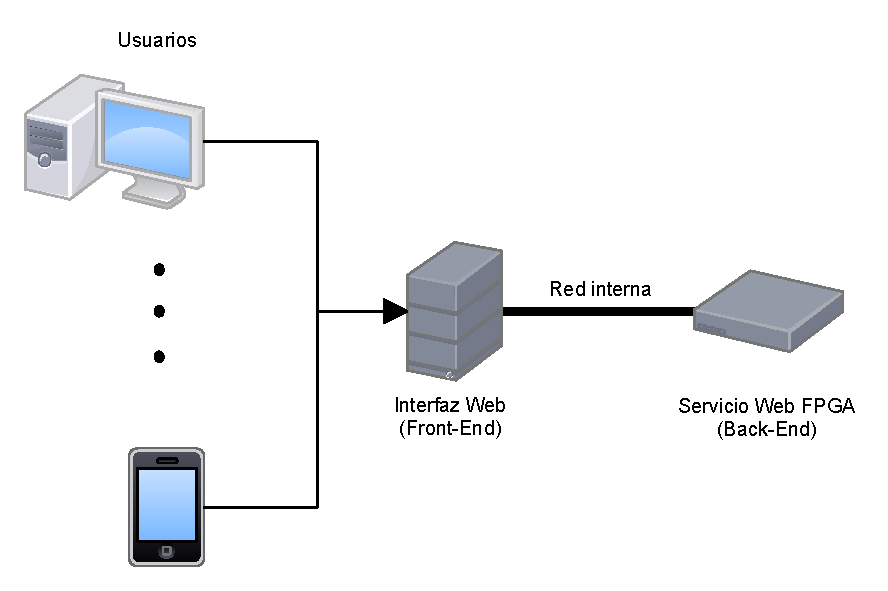
\includegraphics[width=0.9\linewidth]{arquitectura}
  \end{figure}
\end{frame}

% Stack de tecnologías
\begin{frame}{Stack tecnológico}
  \begin{itemize}[<+->]
    \item \alert{Back-End}
    \begin{itemize}
      \item<.-> JavaScript
      \item<.-> node.js
      \item<.-> express, async, nodemon
    \end{itemize}
    \item \alert{Front-End}
    \begin{itemize}
      \item<.-> PHP (HTML, JavaScript, CSS)
      \item<.-> Framework propio
      \item<.-> Bootstrap, jQuery
    \end{itemize}
  \end{itemize}
\end{frame}

% Back-End
\begin{frame}{Back-End}
  \begin{itemize}[<alert@+>]
    \item Servicio Web FPGA
    \item Comunicación con la sonda
    \item Monitorización del sistema
  \end{itemize}
\end{frame}

\begin{frame}{Back-End - Servicio Web FPGA}
  \begin{figure}
    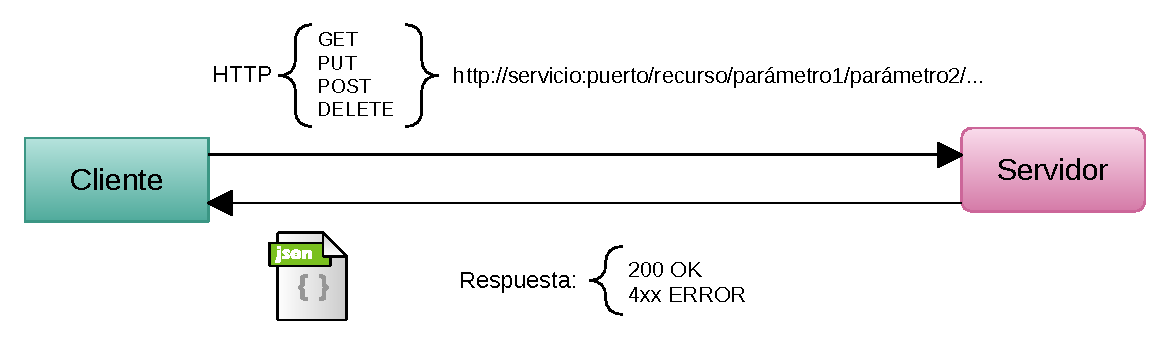
\includegraphics[width=\linewidth]{fpga_rest}
  \end{figure}
\end{frame}

\begin{frame}{Back-End - Arquitectura interna}
  \begin{figure}
    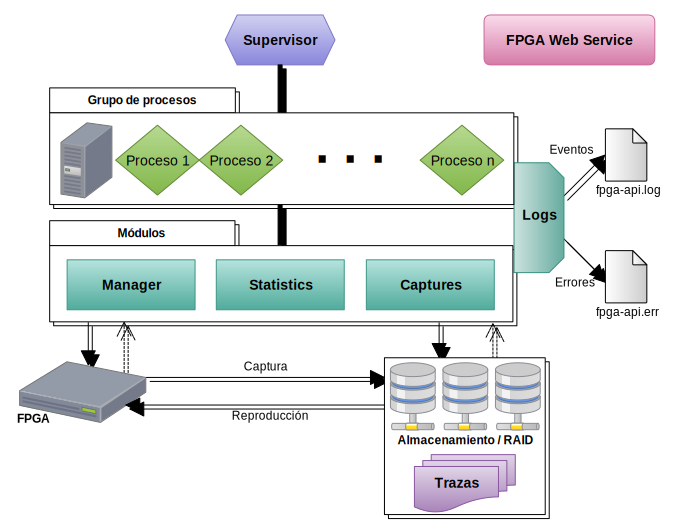
\includegraphics[width=0.85\linewidth]{fpga}
  \end{figure}
\end{frame}

\begin{frame}{Back-End - FSM Estado FPGA}
  \begin{figure}
    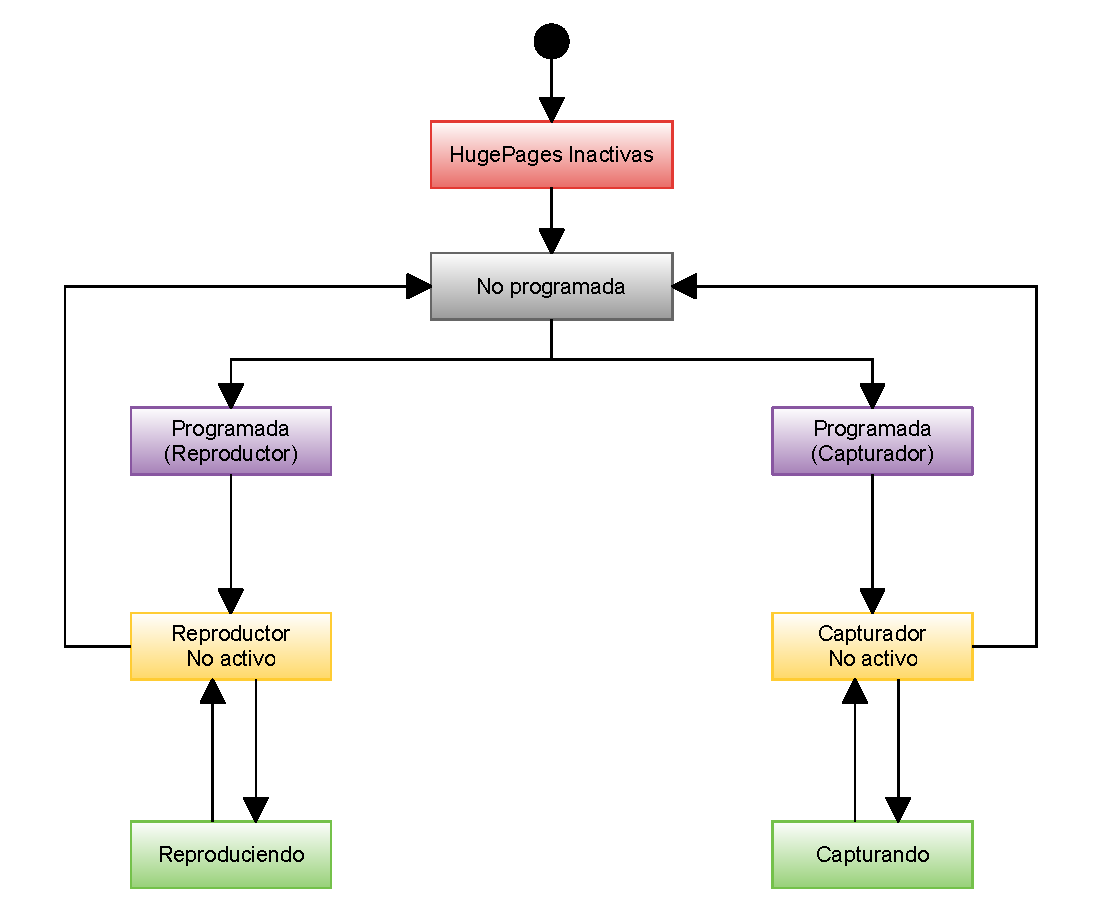
\includegraphics[width=0.8\linewidth]{fpga_estado}
  \end{figure}
\end{frame}

\begin{frame}{Back-End - Determinar estado actual}
  \begin{figure}
    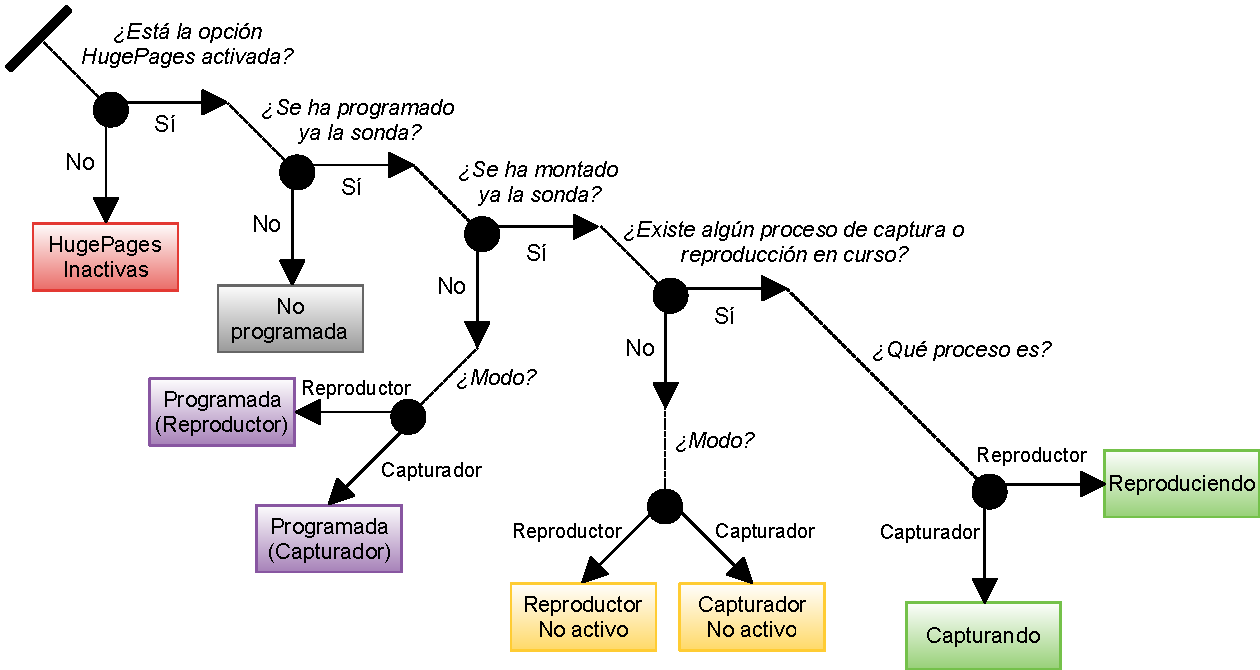
\includegraphics[width=\linewidth]{arbol_decision}
  \end{figure}
\end{frame}

\begin{frame}{Back-End - API REST}
  \begin{figure}
    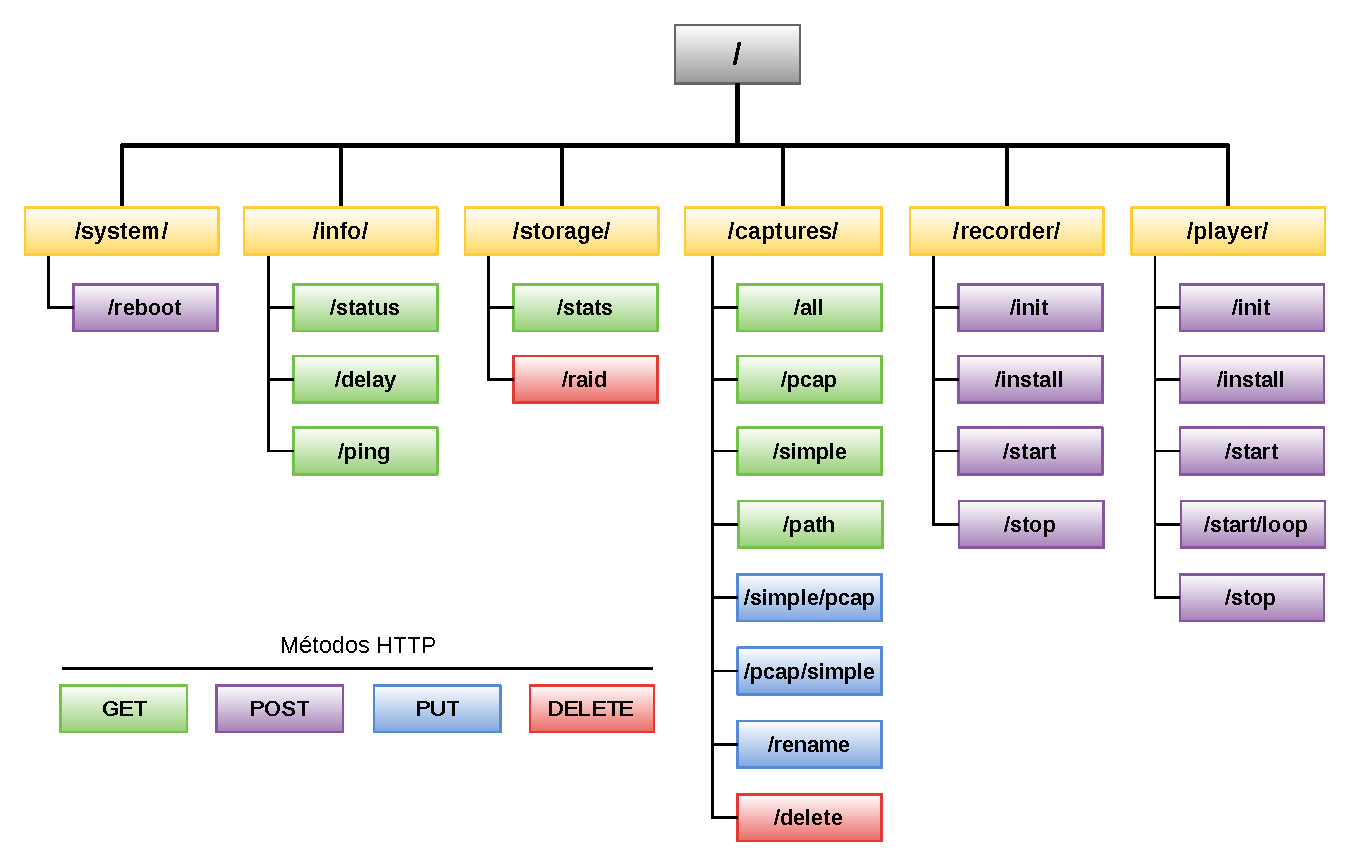
\includegraphics[width=\linewidth]{arbol_metodos}
  \end{figure}
\end{frame}

% Front-End
\begin{frame}{Front-End}
  \begin{itemize}[<alert@+>]
    \item Comunicación con el back-end (proxy)
    \item Framework propio
    \item Diseño \textit{responsive}
  \end{itemize}
\end{frame}

\begin{frame}{Front-End - Framework - Arquitectura interna}
  \begin{figure}
    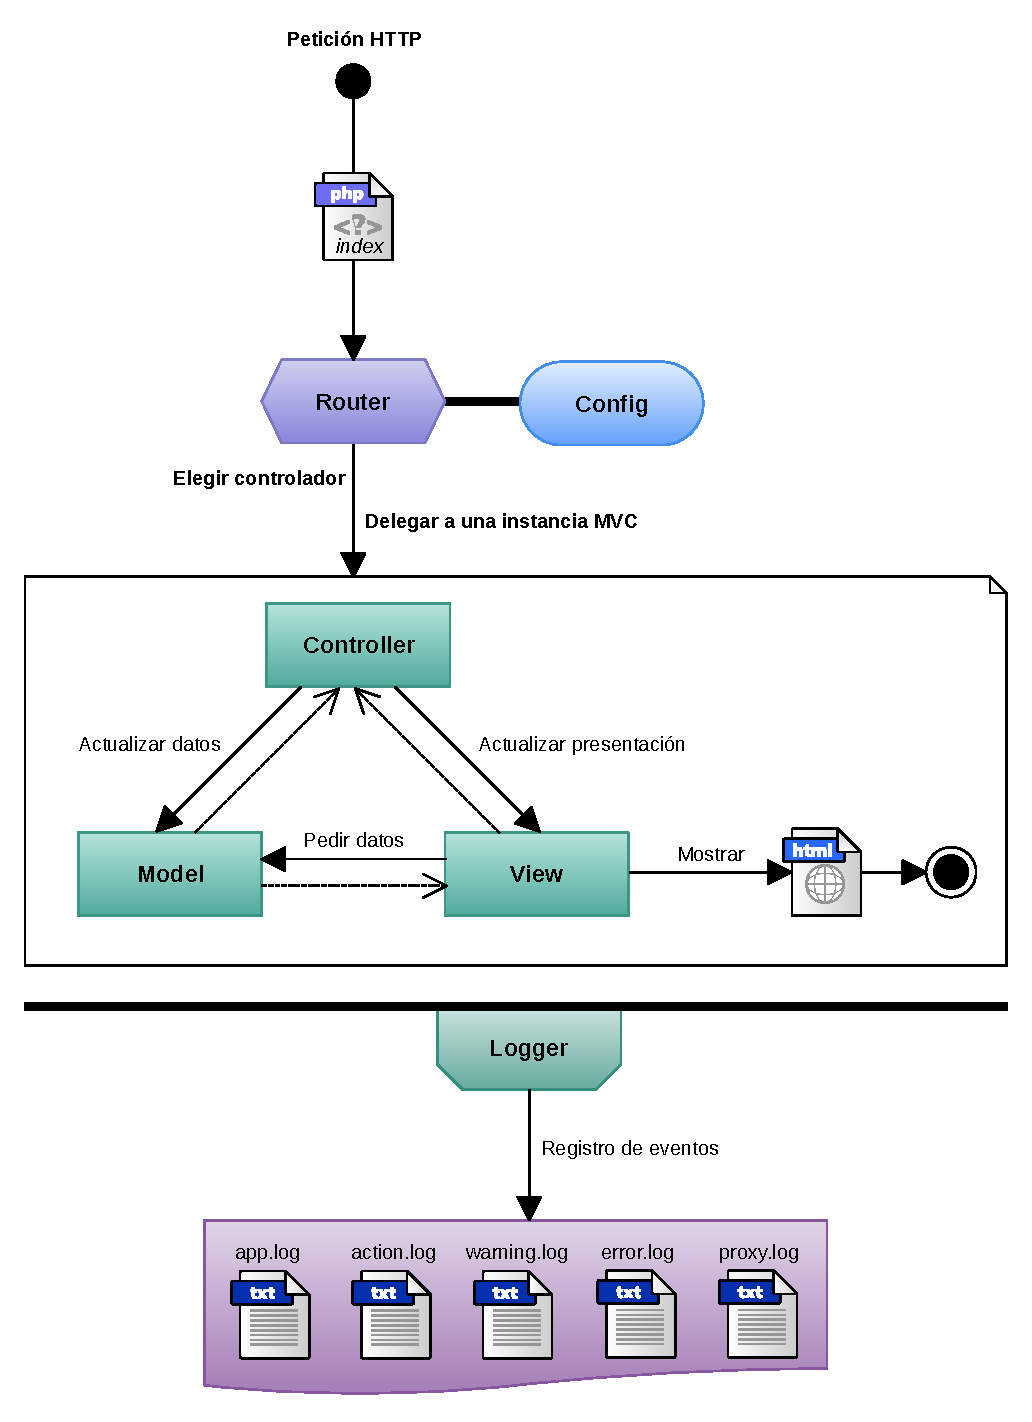
\includegraphics[width=\linewidth]{framework}
  \end{figure}
\end{frame}

\begin{frame}{Front-End - Framework - Router}
  \begin{figure}
    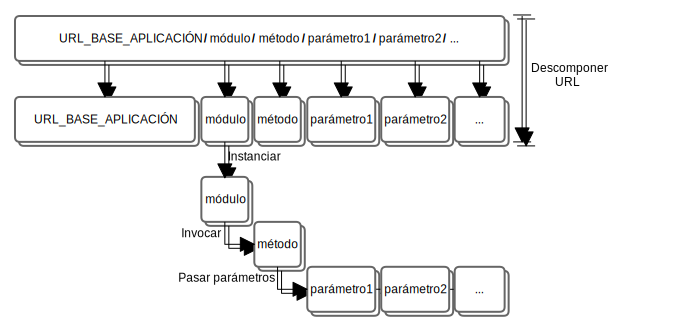
\includegraphics[width=\linewidth]{router}
  \end{figure}
\end{frame}

\begin{frame}{Front-End - Framework - Proxy}
  \begin{figure}
    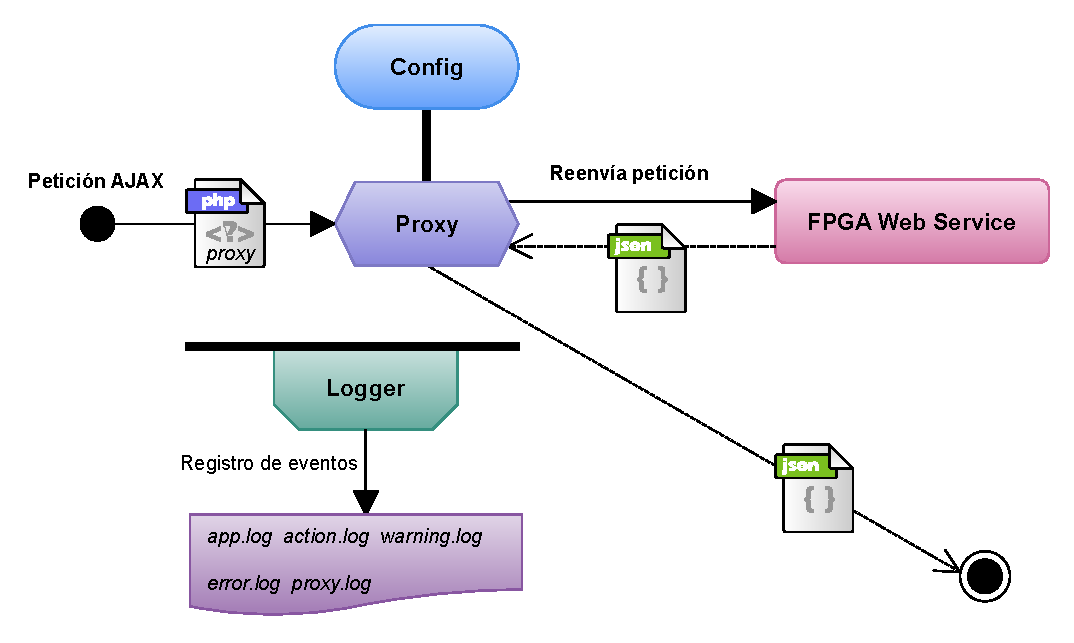
\includegraphics[width=\linewidth]{proxy}
  \end{figure}
\end{frame}

\begin{frame}{Front-End - Diseño - Capturas}
  \begin{figure}
    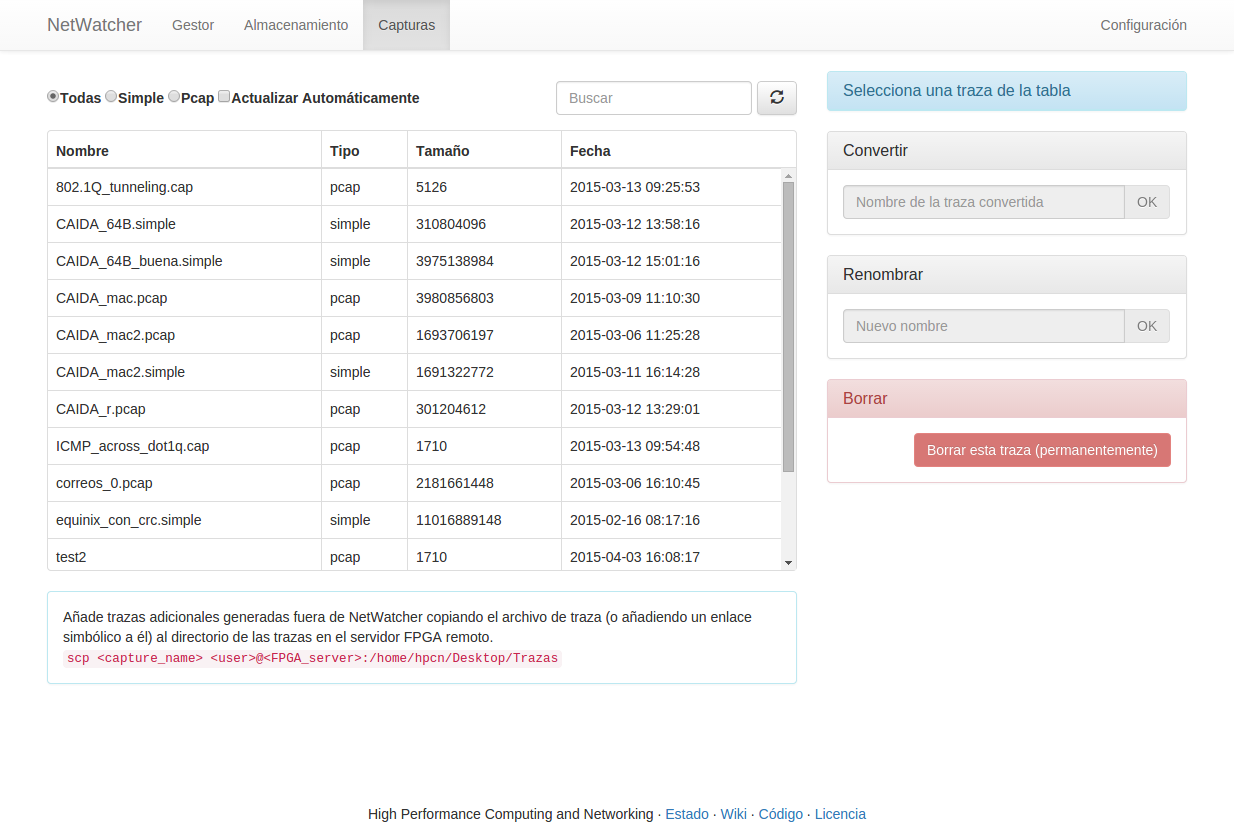
\includegraphics[width=\linewidth]{capturas}
  \end{figure}
\end{frame}

\begin{frame}{Front-End - Diseño - Gestor capturar}
  \begin{figure}
    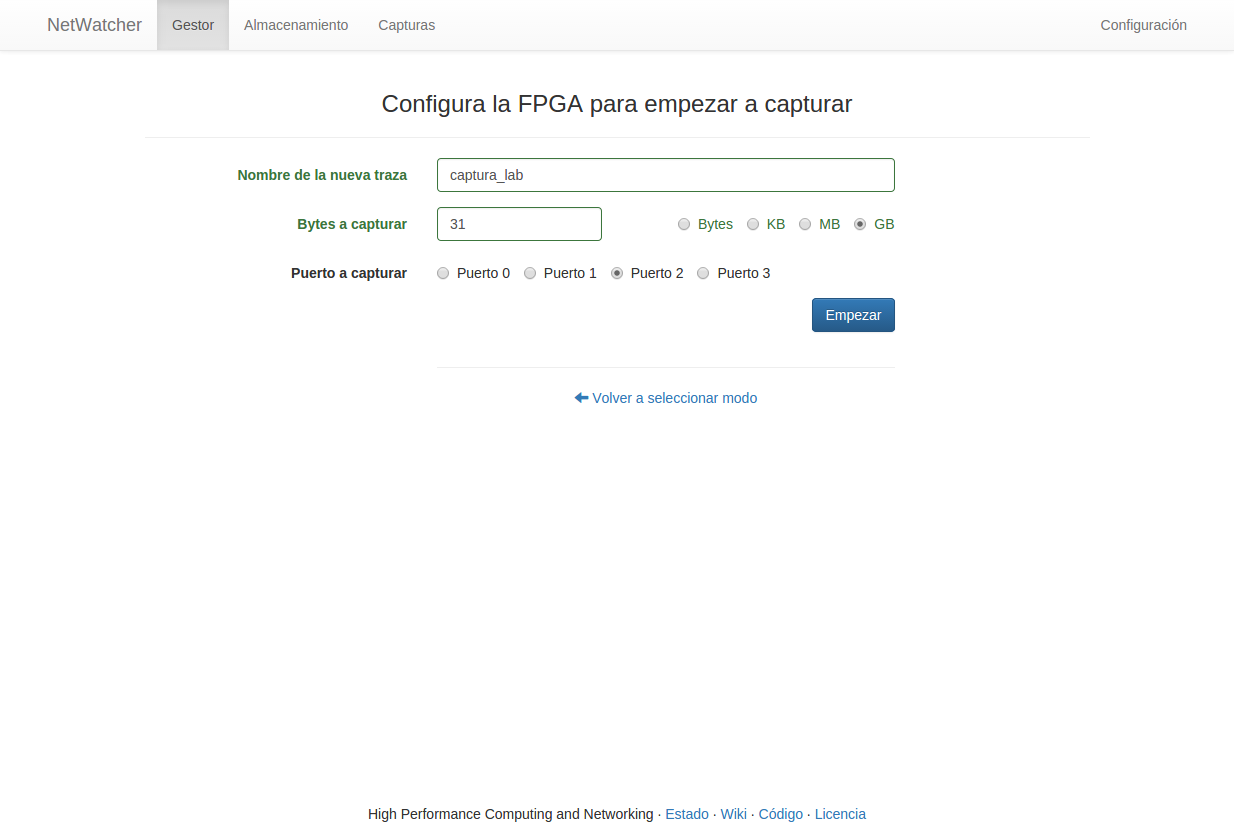
\includegraphics[width=\linewidth]{gestor_capturar}
  \end{figure}
\end{frame}

\begin{frame}{Front-End - Diseño - Estado}
  \begin{figure}
    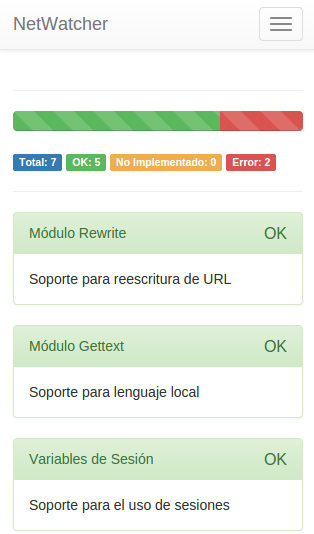
\includegraphics[width=0.3\linewidth]{estado_movil}
  \end{figure}
\end{frame}


% Conclusiones
\section{Conclusiones}

\begin{frame}{Conclusiones}
  \begin{itemize}
    \item Gestión del sistema completo mediante una interfaz web
    \begin{itemize}
      \item Control de la FPGA de forma intuitiva
      \item Administración de las trazas
    \end{itemize}
    \item Trabajo extensible a otras sondas de red
    \begin{itemize}
      \item Arquitectura base
      \item Módulos independientes del modelo de sonda
    \end{itemize}
  \end{itemize}
\end{frame}

\begin{frame}{Contribuciones}
  \begin{itemize}
    \item Proyecto disponible en GitHub
    \begin{itemize}
      \item Liberado bajo licencia MIT
      \item Documentación extensiva
    \end{itemize}
    \item Proyecto europeo de federación Fed4FIRE
    \begin{itemize}
      \item Integración con el testbed de la FPGA
    \end{itemize}
    \item The Open Source Network Tester
    \begin{itemize}
      \item Posible incorporación de la interfaz desarrollada
    \end{itemize}
  \end{itemize}
\end{frame}


% Líneas de Trabajo Futuro
\section{Líneas de Trabajo Futuro}

\begin{frame}{Líneas de Trabajo Futuro}
  \begin{itemize}[<alert@+>]
    \item Extensión a más sondas de red
    \item Módulo de autenticación
    \item Soporte a más tipos de trazas
    \item Registro de estadísticas adicionales
    \item Interfaz en otros idiomas
  \end{itemize}
\end{frame}


% Agradecimientos
\section{Agradecimientos}

\begin{frame}{Agradecimientos}
   TODO: Agradecimientos (Sergio/HPCN)
\end{frame}


% Preguntas
\plain{¿Preguntas?}

\end{document}
